\section{Proof-of-Concept Attack}
\label{sec:poc.attack}

\subsection{Test bed Setup}
\label{sec:attack.setup}

As proof of concept, and illustrative strawman for the weakness of RDMA we
perform a man-in-the-middle attack. We demonstrate the power that an attacker
with the ability to read and modify packets in the network can wield. For
simplicity, and due to our lack of access to s specialized router that supports
packet eavesdropping and manipulation, we used \texttt{scapy} to emulate router
on a regular Ubuntu server.

\begin{figure}[ht]
    \centering
    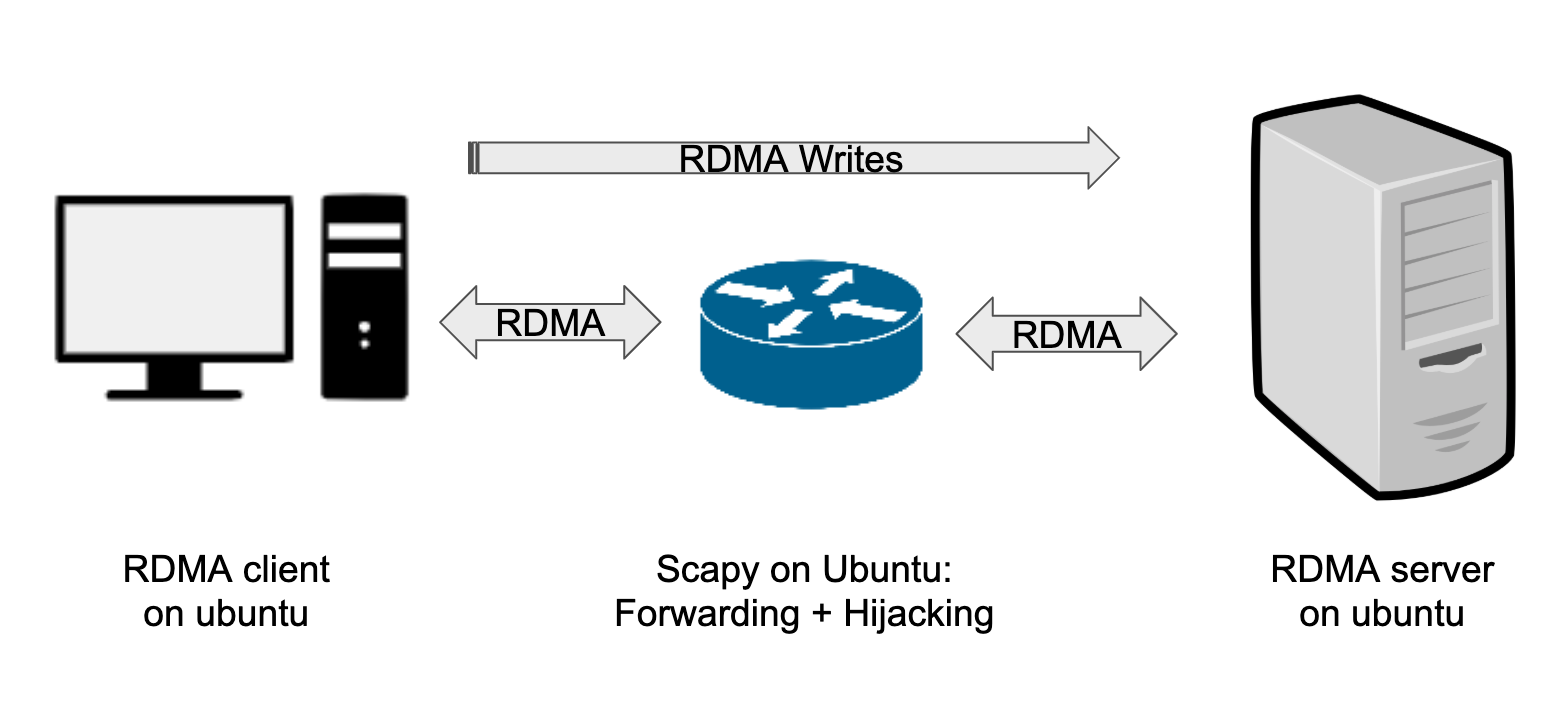
\includegraphics[width=0.5\textwidth - 5pt]{fig/attack_setup}
    \caption{Attack Testbed Setup}
    \label{fig:attack.setup}
\end{figure}

We run a RoCEv2 RDMA client and server on two Ubuntu servers as seen in
Figure~\autoref{fig:attack.setup}. Both client and server are connected to an
attacker machine in the middle which uses \texttt{scapy} to sniff all
\texttt{RoCEv2} packets, re-write the MAC addresses and forward it to an egress
port. During attacks we allow the attacker to modify the packet as needed, after
which we re-compute the \texttt{RoCEv2} checksum according to the IBTA specs
\cite{infiniband:iba.spec.vol1.v1.3}, RoCE annex
\cite{infiniband:iba.spec.annex.roce} and RoCEv2 annex
\cite{infiniband:iba.spec.annex.rocev2}.

We set up the \texttt{ARP} entries manually such that both client and server
think they are talking to the each other directly, but in reality, the packets
will all go through the middle machine. This configuration simulates a
compromised switch in which an attacker has gained control over the data plane
and can advertise arbitrary MAC address to connected hosts.

\texttt{scapy} is a \texttt{Python} module that allows packet sniffing,
manipulation, injection, etc.  It internally calls \texttt{tcpdump} and works on
raw socket as well, which gives us the ability to re-write Ethernet-layer MAC
addresses.

\subsection{The RDMAttack }
\label{sec:attack.model}

For our proof-of-concept attack, we choose to hijack the write address of RDMA
write requests. Gaining control over a write location allows an attacker to
place arbitrary data in a victims address space. Additionally it allows an
attacker to seer RDMA traffic to select locations which can be used for
Throwhammer exploits. We chose write as it gives the attacker explicitly more
control over the victim. RDMA verbs for write are identical to reads, for the
sake of brevity we could have modified read address and read sizes. This attack
while omitted could be used to cause a victim to flood the network with
Terabytes of unrequested data.

\begin{figure}[h]
    \centering
    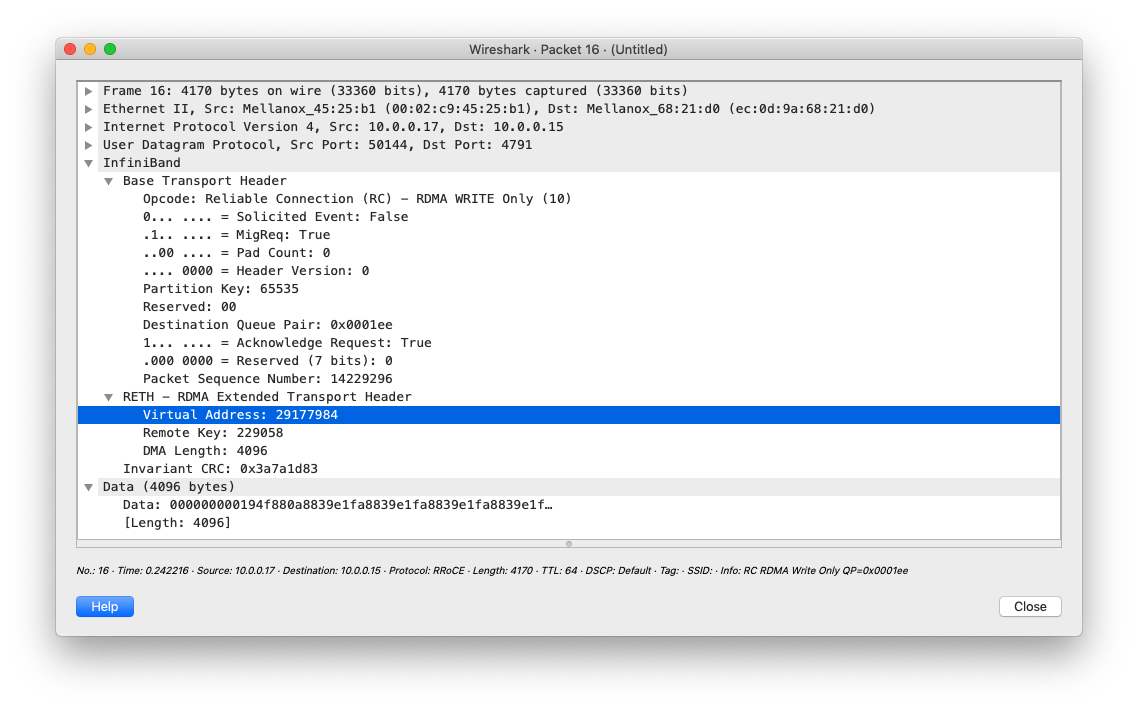
\includegraphics[width=0.5\textwidth - 5pt]{fig/rdma_write_packet_wireshark}
    \caption{RDMA Write Packet in Wireshark}
    \label{fig:attack.rdma_write_packet}
\end{figure}

RDMA WRITE allows the requestor/client to write data to the address space of the
target application on the target machine / server, using a remote key negotiated
via prior authentication. Neither the key nor the virtual address is encrypted,
as show in \autoref{fig:attack.rdma_write_packet}.

We decided to hijack all writes to the same address, which can be handy to carry out Throwhammer attack
as previously shown \cite{216055}.
For our PoC, our adversary remembers the virtual address of the first WRITE it sees,
and changes addresses of all subsequent WRITEs to be the same.

\subsection{RDMA Client/Server}
\label{sec:attack.rdma_app}

For simplicity, our RDMA client will issue $n$ RDMA WRITE requests after initial handshake and
information exchange needed for one-sided RDMA operations like RDMA WRITE. According to the attack model
described in \autoref{sec:attack.model}, our attacker hijacks all subsequent RDMA WRITEs. Thus, we compare:
1) client issues on RDMA write, and 2) client issues two RDMA writes to two different address.

We used a modified RDMA performance benchmark tool, which in the first case, issues one RDMA WRITE of 16 bytes,
and the second case, issues two consecutive RDMA WRITEs of 16 bytes each. At the end, both client and server
computes the SHA1 checksum of the buffer region. If the SHA1 digest matches, then it means all data have been
transferred successfully and not been tampered with.

\begin{table*}[ht]
    \begin{tabular}{c|c|c}
        Experiment \# & $1$ & $2$ \\ \hline
        SHA1 digest (client) & 609f05f73fb251aec1c7d8b25b4cbe1d2d1a1661 & b262a891b5dfc43930d6aa733e9741e625126a89 \\
        SHA1 digest (client) & 609f05f73fb251aec1c7d8b25b4cbe1d2d1a1661 & 2488224f4d0dff339e01d1694a0bee162eb8c358 \\
    \end{tabular}
    \caption{RDMA Proof-of-Concept Result}
    \label{table:attack.result}
\end{table*}

\subsection{Result}
\label{sec:attack.result}

As show in \autoref{table:attack.result}, in the first case, there is only one RDMA WRITE, so the attacker doesn't
modify the requests at all, thus the SHA1 digests match. But in the second case, since there are two RDMA writes, the
second RDMA WRITE is hijacked so the buffer for the second WRITE did not complete successfully. Thus the SHA1 digests
don't match. This simple proof-of-concept shows that it is (very) possible for attackers who compromised a switch to
carry out RDMA attacks like Throwhammer and more.
